\documentclass{article}
\usepackage[utf8]{inputenc}
\usepackage{amsmath}
\usepackage{amsfonts}
\usepackage{graphicx}

\title{Discussion Assignment Unit 5\\
Math 1201- College Algebra.
}
\author{Jasper Albert Nri}
\date{October 2021}


\begin{document}

\maketitle

\section*{Logistic Equation}
The population of a culture of bacteria is modeled by the logistic equation.
$${p(t) = \frac{14250}{1+29e^{-0.62t}}}$$ 
\title\textbf{Solution}
According to Abramson(2017). The logistic growth model is
$${f(x) = \frac{c}{1+ae^{-bx}}}$$
where 
\\${\frac{c}{1+a}}$ is the initial value
\\c is the carrying capacity, or limiting value.
\\b is a constant determined by the rate of growth.\\
\\\title\textbf{Carrying Capacity}\\ 
Going by this the carrying capacity, c of the population of the culture of bacteria is 14250.\\ 
\\\title\textbf{Initial Population}\\ 
The initial Population of the culture is given by 
$${\frac{c}{1+a} = \frac{14250}{1+29}}$$
$${\frac{c}{1+a} = 475}$$
\\\title\textbf{Days to reach 75\% of its carrying capacity }\\ 
Equating 75\% of the carrying capacity to the logistics function.\\
$${.75(14250)= \frac{14250}{1+29e^{-0.62t}}}$$
Dividing both the LHS and RHS by 14250
$${.75= \frac{1}{1+29e^{-0.62t}}}$$
Rearranging the equation
$${1+29e^{-0.62t}= \frac{1}{.75}}$$
$${29e^{-0.62t}= \frac{1}{.75} - 1}$$
$${29e^{-0.62t}= \frac{4}{3} - 1}$$
$${e^{-0.62t}= \frac{1}{3\times29}}$$
$${e^{-0.62t}= \frac{1}{87}}$$
Taking the natural log of both sides
$${-0.62t= \ln\left(\frac{1}{87}\right)}$$
Dividing both the LHS and RHS by -0.62
$${t= \frac{\ln\left(\frac{1}{87}\right)}{-0.62}}$$
$${t= 7.2}$$
\\Therefore it would take this logistic equation 7.2 days to reach 75\% of its carrying capacity.\\\\
\\\title\textbf{${P(t) = P_{0} e^{kt}}$}
\\A model like ${P(t) = P_{0} e^{kt}}$ is an exponential growth model and it would not be plausible for modelling the population of a culture of bacteria because the exponential function represents unlimited exponential growth and this does not model reality, because in reality the culture of bacteria will eventually slow down in its growth rate, because there is a finite amount of resource available to facilitate it's growth (Abramson, 2017).\\ 
\\The most important virtue of the logistic model is that it models reality by imposing an upper bound called its carrying capacity, which caps of the growth rate and prevents the model from increasing indefinitely exponentially(Abramson, 2017). 



The graph of the logistic model is shown below\\
$${y\ =\frac{14250}{\left(1+29\cdot e^{\left(-0.62\cdot x\right)}\right)}\ \ \left\{0<x<15\right\}\left\{0<y<15000\right\}}$$
$${y=\ 14300\ \left\{0<x<15\right\}}$$
\\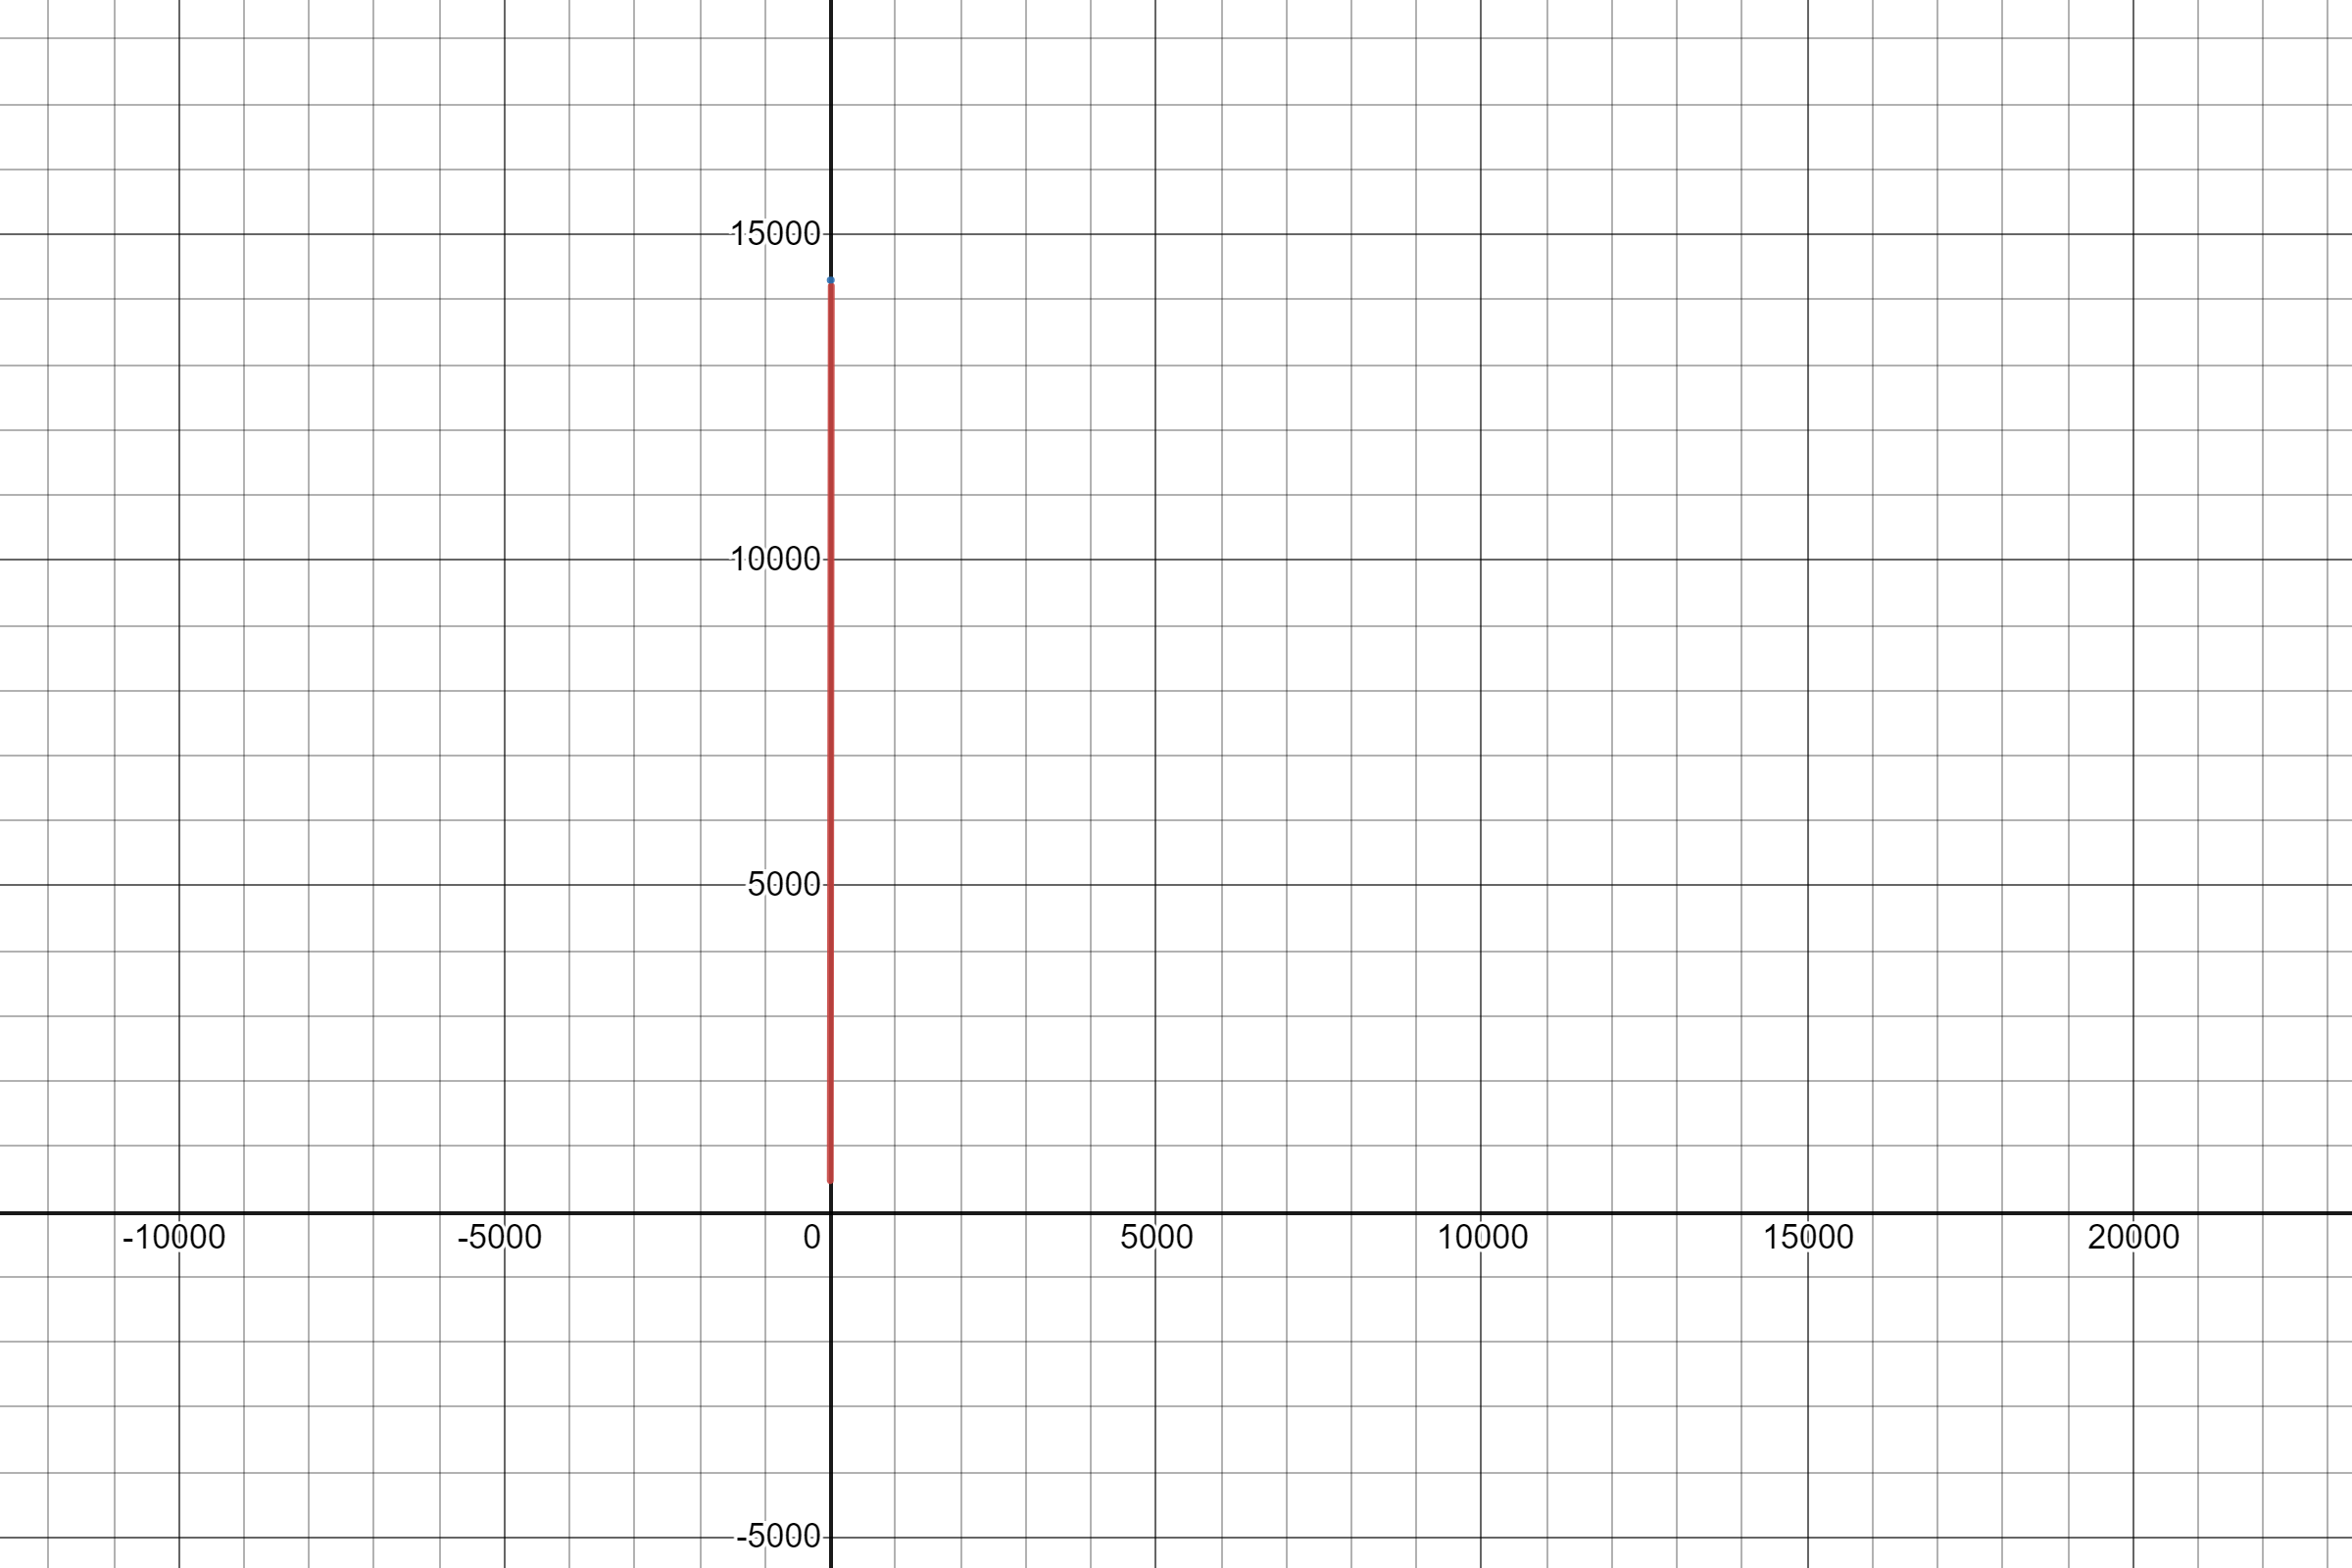
\includegraphics[scale = 0.1]{p1}\\
\\At the endpoint of the graph
\\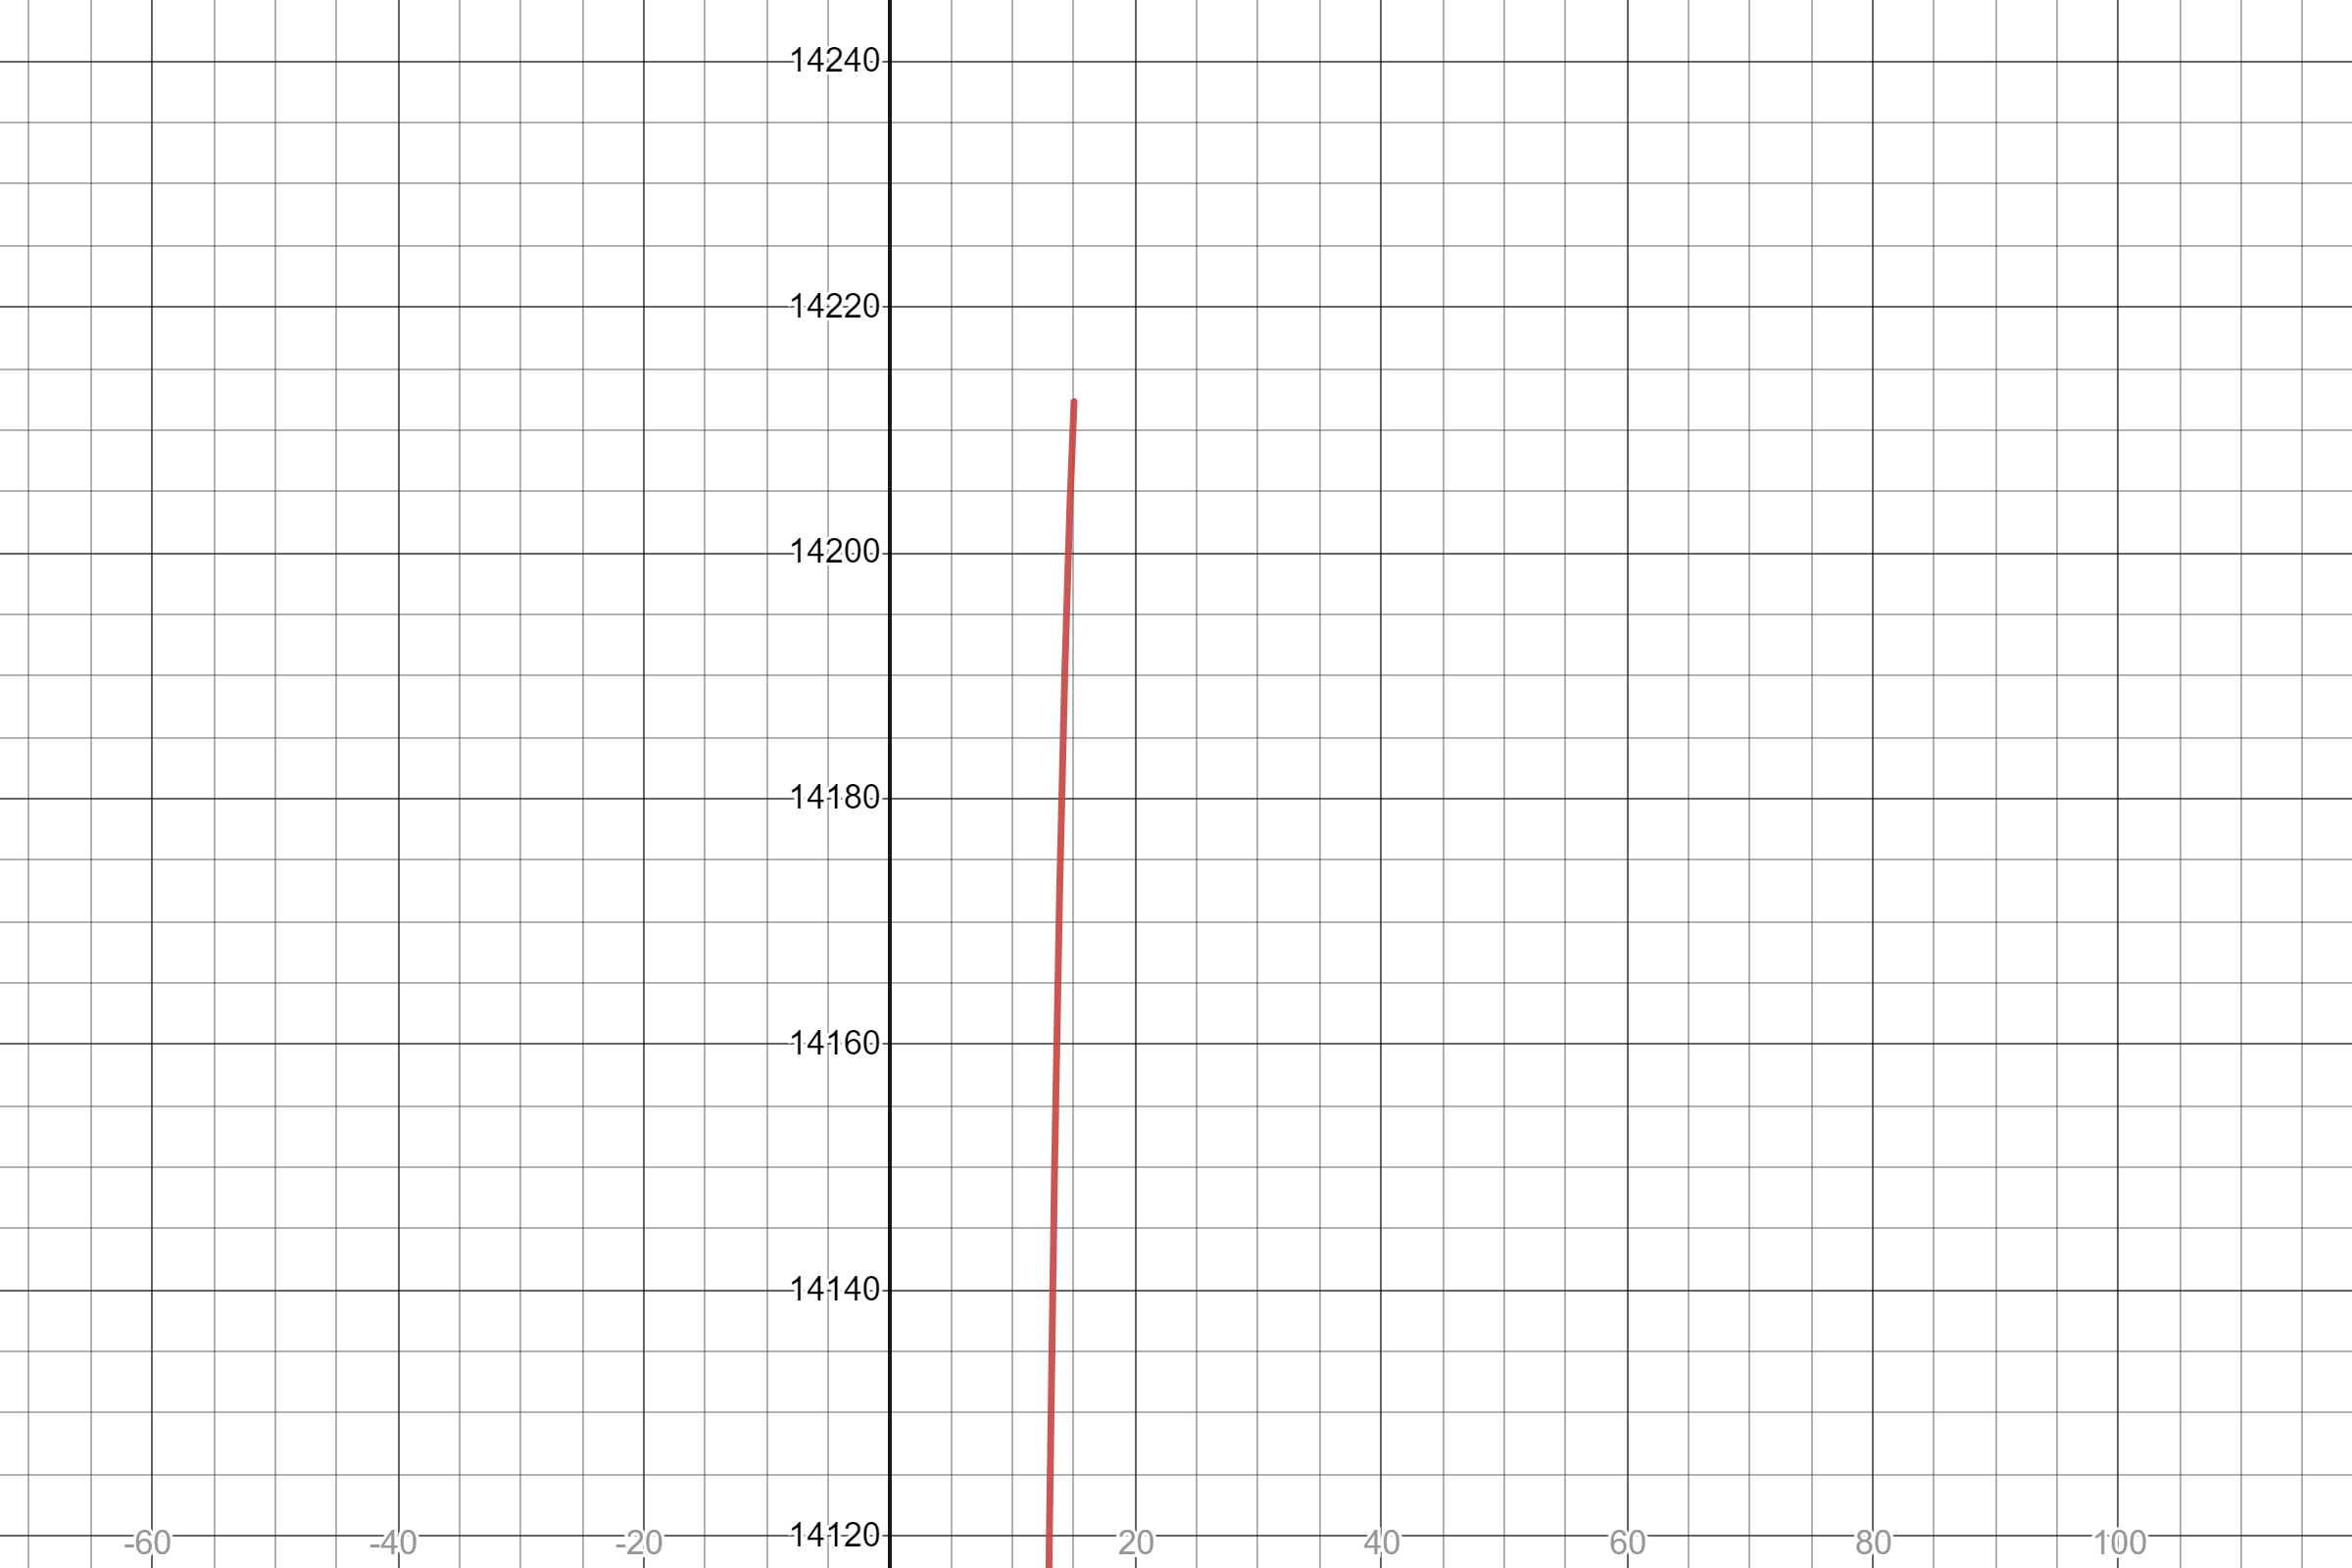
\includegraphics[scale = 0.1]{p2}\\
\\I used the desmos graphing calculator to obtain this graph.
\section*{REFERENCES}
Abramson, J. (2017). \textit{Algebra and trigonometry}. OpenStax, TX: Rice University. Retrieved
from https://openstax.org/details/books/algebra-and-trigonometry
\end{document}